\section{Notes to Oriental Metaphysics}

I've been cleaning up paperwork. I stumbled across some personal musings that go back decades. The topics then are similar to those of today, although the approach was quite different. I also found some class notes for a discussion group on Oriental Metaphysics by Rene Guenon. They date back to November 2005. The audience was primarily Theosophists and Vedantists, who had little understanding of metaphysics. The following notes were geared to them. They are merely an introduction to certain concepts. I have only found the notes for the first class. In retrospect, further notes were probably not necessary as we went straight to the text.

\begin{quotex}
The consummation of the infinite End, therefore, consists merely in removing the illusion which make it seem yet unaccomplished. The good, the absolutely Good, is eternally accomplishing itself in the world: and the result is that it needs not wait upon us, but is already by implication, as well as in full actuality, accomplished. This is the illusion under which we live. It alone supplies at the same time the actualizing force on which the interest in the world reposes. In the course of its process the idea creates that illusion, by setting an antithesis to confront it; and its action consists in getting rid of the illusion which it has created. Only out of this error does the truth arise. In this fact lies the reconciliation with error and with finitude. Error or other-bine, when superseded, is sill a necessary dynamic element of truth; for truth can only be where it makes itself its own result.

\flright{\textsc{Hegel}, \emph{Logic}}

The dominant note of barbarism is will and that of culture, especially the culture influenced by Greek ideas, is reason or intellect, so that of Christendom is love.

\flright{\textsc{Martin D'Arcy}, \emph{The Mind and Heart of Love}}

\end{quotex}
\paragraph{Aporia}
Aporia is an insoluble contradiction or paradox in a text's meanings. (The end result of dialog.)

\paragraph{Stages of Rationality}
\begin{wrapfigure}{rt}{0.35\textwidth}
 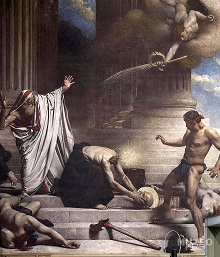
\includegraphics[scale=.7]{a20201222NotestoOrientalMetaphysics-img001.jpg} 
\caption{Losing one's head, finding ones' heart}
\end{wrapfigure}

\begin{itemize}
\item \textbf{Subrational.} The subrational is characterized by instinct, impulse, elan vital, unchecked will. Lacking an inner check or desires, subrational societies rely on custom and taboo to control behaviour. These often seem quite irrational to outsiders. 
\item \textbf{Rational.} Reason gives man much power of nature, and to a lesser extend, over his own passions. However, every assertion creates its opposite, every Yes a No, every Idea its antithesis. These antinomies result in interminable — and irresolvable — discussions. “Reasonable men can agree to disagree”, which demonstrates, not the value of reason, but its impotence to lead to any kind of genuine knowledge. 
\item \textbf{Surparational.} The suprational, or metaphysical intuition, is above reason, yet not irrational. Dualities are resolved, and there is a genuine knowledge (gnosis). Identifying characteristics are: 

\begin{enumerate}
\item Conforms to experience 
\item Coherent 
\item Consistent with natural knowledge 
\end{enumerate}
\end{itemize}
\paragraph{Occam's Razor}
\emph{One should not increase, beyond what is necessary, the number of entities required to explain anything.}

It is necessary to resist the temptation to postulate entities such as “higher” and “lower” minds, etc. The fundamental insight is to realize the unchanging and eternal that subtends every experience. This is the Witness, or Self, which is \emph{not} a postulated entity, since it can never be an “object” to anything.

Reading a work like Oriental Metaphysics is in invitation to achieve such self-realization.

\paragraph{Degrees of Experience}
Here are some distinctions to keep in mind:

\begin{itemize}
\item \textbf{Metaphysical Intuition}. This is the realization of the Atman, Self, Witness. It is beyond any particular state of being, and beyond any particular experience. It is beyond nature. 
\item \textbf{Mystical Experience}. This is an experience of a state of being higher than the human state. Although such experiences may be rapturous, ecstatic, extraordinary, insightful, and peaceful, they still belong to the phenomenal realm. This is what distinguishes such an experience from metaphysical intuition. 
\item \textbf{Paranormal Experience}. This is an experience of the subtle (i.e., non-physical) realms of the human state. 
\item \textbf{Demonic Experience}. “Demons” are particular constellations of thought patterns that can influence behavior. Since the ego often identifies with such patterns, it considers them its own, and is in bondage to them. As such, this is akin to “demonic possession”. 
\end{itemize}
Guenon is careful to strongly distinguish Metaphysical Intuition from particular experiences. Mystical and paranormal experiences are still in the psychic or psychological realm.

\paragraph{Characteristic Signs}
\begin{itemize}
\item \textbf{Ataraxy}. Tranquility, imperturbability. State of soul which is peaceful, undisturbed by events, either external, or even internal, such as thoughts, fantasies, desires, emotions. 
\item \textbf{Apatheia}. This is not the Stoic state of freedom from emotions, but rather freedom from “passions”, rightly understood. They are negative emotions contrary to nature (not nature just limited to the physical!). Examples: conceit, gluttony, lust, vanity, greed, malice. Some emotions may or may not be contrary to nature, depending on their object: anger, hatred, sorrow, fear.

Similarly, some legitimate pleasures and desires are not necessarily passions. One obvious example is the feeling of Bliss (Ananda) which accompanies metaphysical realization. 
\item \textbf{Agape}. More than friendship, family affection, or erotic attraction. This is spiritual love. 
\end{itemize}
\paragraph{Lessons to be Learned}
It has been said that life is a school, where lessons are to be learned. If so, it is a strange sort of school where we are not only not given the answers to the question, we are not even given the questions. If lessons are to be learned, we seldom see it. Instead there are the same mistakes repeated, plans gone awry, potentials unfulfilled, resolutions broken, love unrequited.

Desire is insatiable, no sooner is one fulfilled, than a dozen others arise to take its place. If there is a lesson to learned, it must be this:

There is no solution within life.

Isn't this also Buddha's conclusion, or Jesus' assertion that “My kingdom is not of this world”? The solution is in another direction, unnatural, or better, supernatural (in the true meaning of this term). Therein lies deliverance.

Only the human state offers the possibility for deliverance (or Beatific Vision).

\paragraph{One Thing Needful}
With it, there is not doubt; without it, there is no understanding.

This is the realization of the Self that witnesses, but is not witnessed.

Prakriti (matter) brings into manifestation (multiplicity) Purusha (spirit).

What does the Witness witness when it is witnessing?



\flrightit{Posted on 2020-12-22 by Cologero }
